% Intended LaTeX compiler: pdflatex
\documentclass{scrartcl}
		\usepackage[utf8]{inputenc}
    \usepackage[dvipdfm]{geometry}
		\usepackage[dvipdfmx]{graphicx}
		\usepackage[dvipdfmx]{color}
		\usepackage[backend=biber,bibencoding=utf8]{biblatex}
		\usepackage{url}
		\usepackage{indentfirst}
		\usepackage[normalem]{ulem}
		\usepackage[dvipdfmx]{hyperref}
		\usepackage{longtable}
		\usepackage{minted}
		\usepackage{fancyvrb}
		
		\bibliography{reference}
\author{情報科学類二年 江畑 拓哉(201611350)}
\date{}
\title{seis-ml-api}
\begin{document}

\maketitle

\section{全体案}
\label{sec:org6323aaf}
 以降この図に記載された名称を用いて説明を行う。\\
\begin{figure}[htp]
  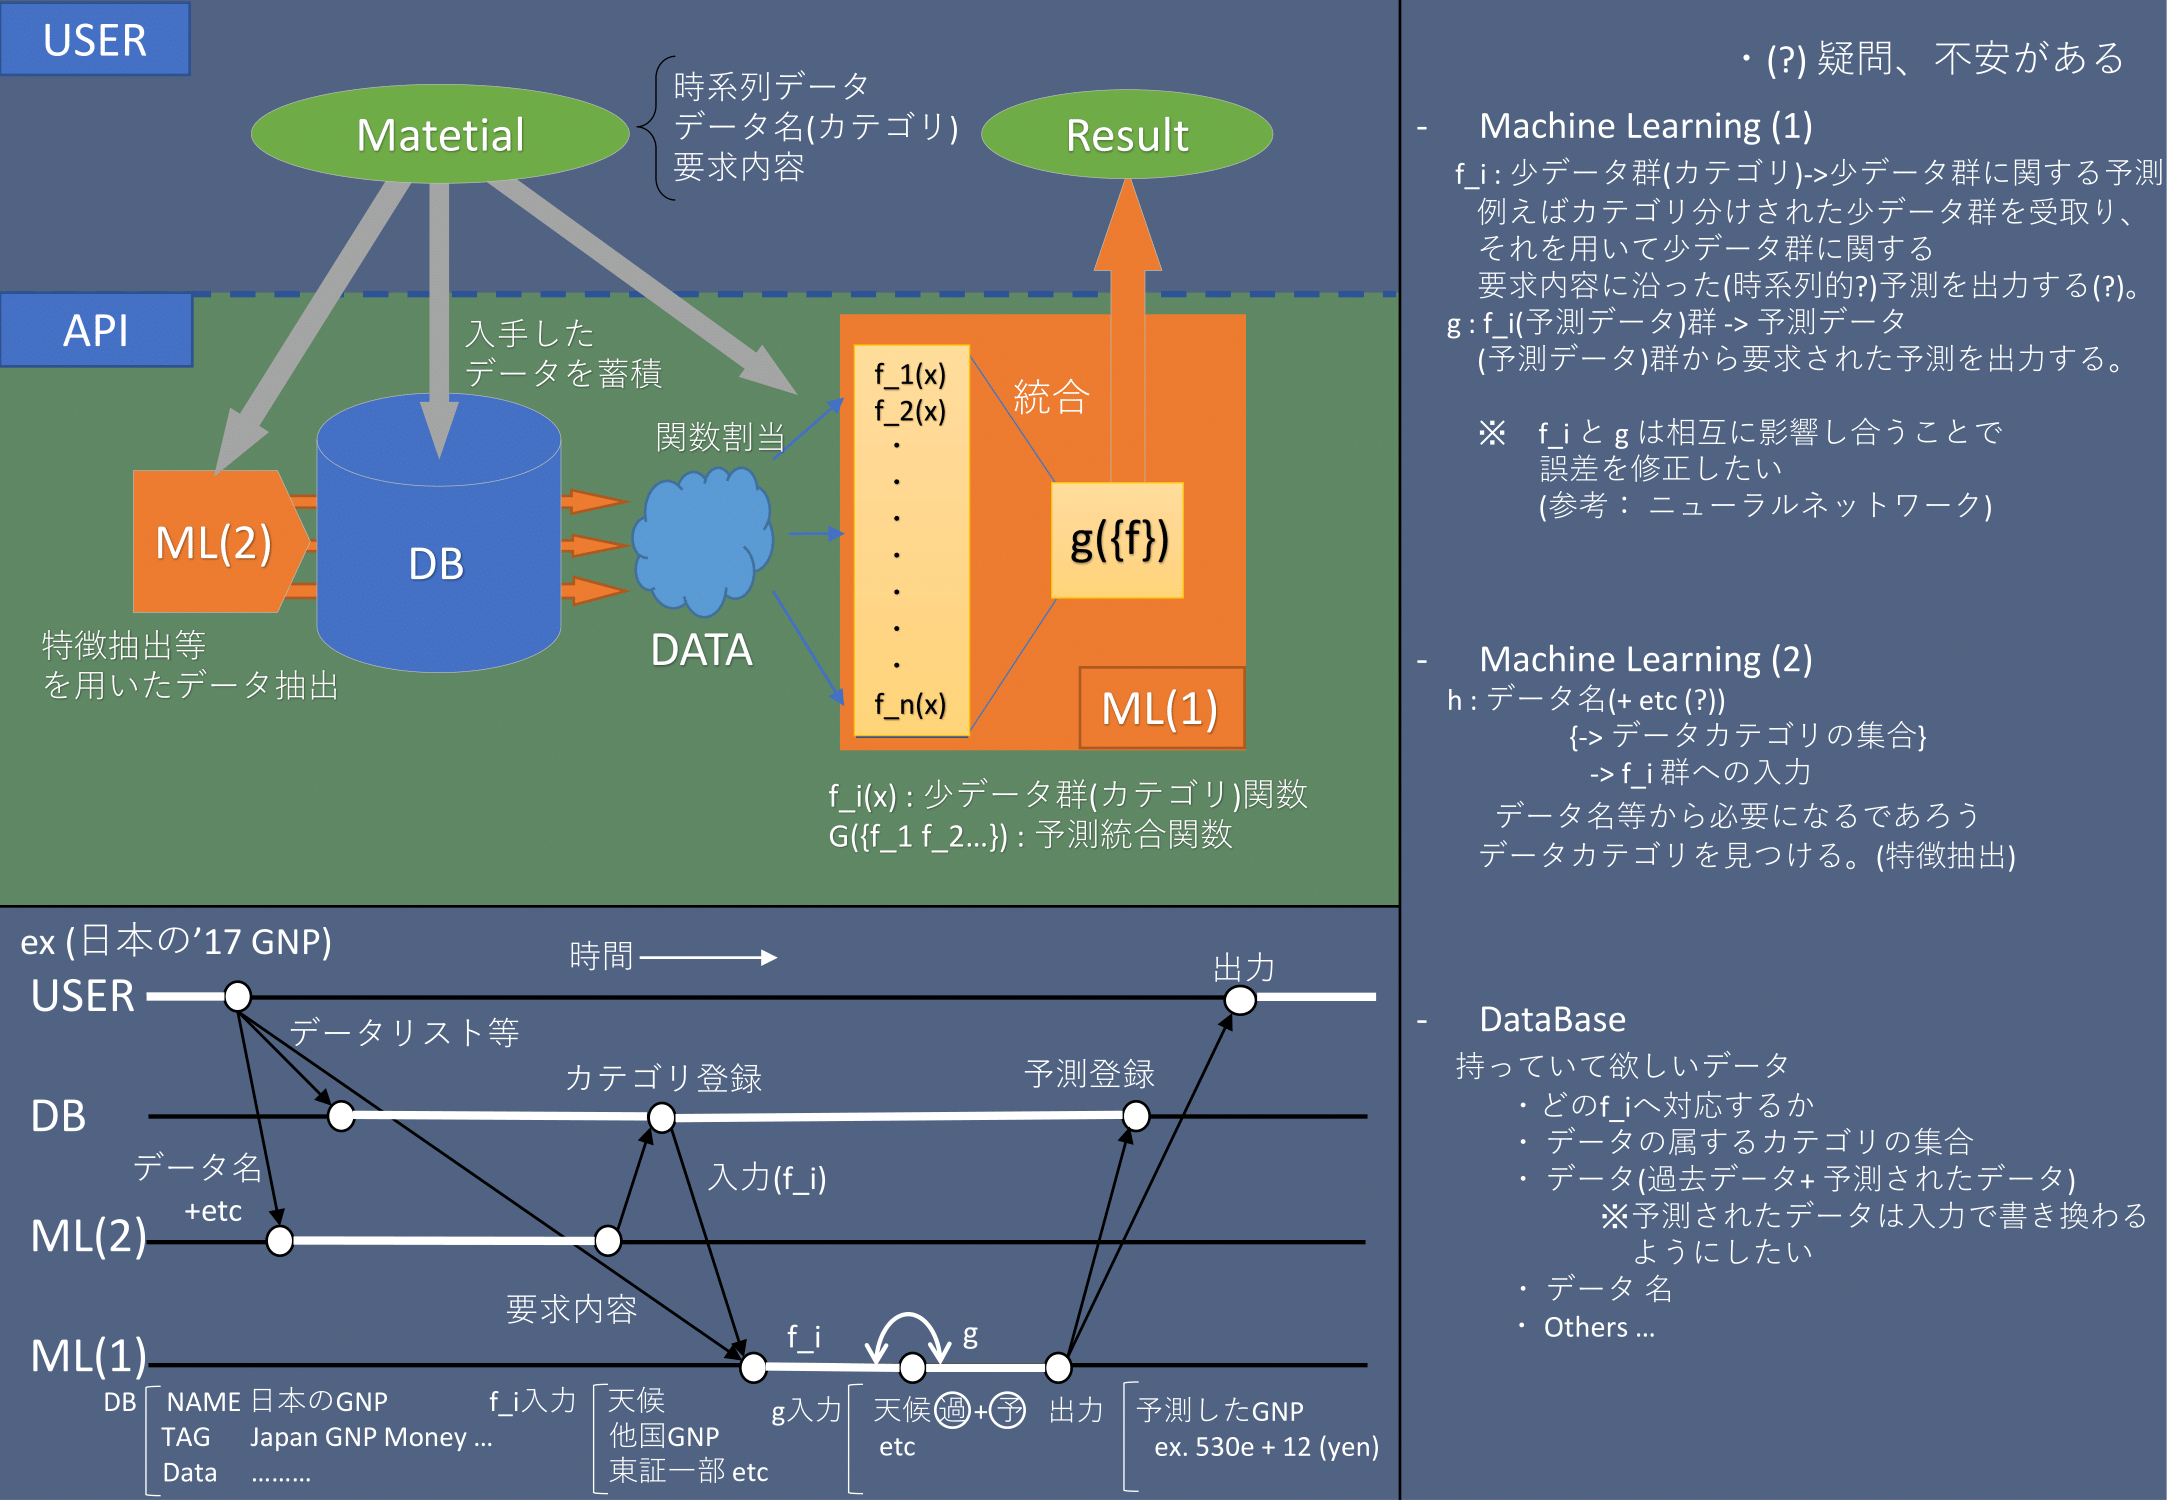
\includegraphics[width=15cm]{./idea-0-1.png}
\caption{全体案}
\end{figure}

\section{機械学習部分(1)}
\label{sec:orge24aa4b}
 メインとなる機械学習部分Machine Learning(1)については回帰アルゴリズム又はランダムフォレストと重回帰分析を用いたいと考えている。そのうち、非線形回帰分析又はランダムフォレストに関しては、f\_i関数部分で用いたいと考えている。同様に、重回帰分析については、g関数部分で用いたいと考えている。\\
\textit{<2017-07-17 月> } f\_i関数についてはランダムフォレスト、g関数については重回帰分析を行いたいと考えている。\\
\subsection{回帰分析}
\label{sec:org52a4efc}
一般的なアルゴリズムには以下の種類がある。 \cite{kobe-u01}\\
\subsubsection{線形回帰}
\label{sec:org40e65cf}
\begin{itemize}
\item 一般化線形モデル\\
 分布関数に残差が従っている場合に用いることができる。よって複数の分布族でこれを試し、最適な分布を選び出していくのだろうと考えられる。これが元になって、ロジスティック回帰、ポアソン回帰などが含まれている\\
\item ロジスティック回帰\\
ベルヌーイ分布に従う変数の統計的回帰モデルである。ベルヌーイ分布とはそもそも確率 \(p\) で1を確率 \(q=1-p\) で0を取る離散分布 (\(f(k;p)=p^k*q^{1-k}\)) である。これはクラスタリング(教師なし)や分類(教師あり)に用いる方が有用であるようで、そちらの例のほうが多く見受けられた。\\
モデルは以下の通りである。\\
 \(y = \alpha / (1 + \beta * exp(-x*y) )\)\\
\end{itemize}
\subsubsection{非線形回帰}
\label{sec:orgda07480}
\begin{itemize}
\item 多項式回帰\\
線形回帰を曲線にしたもので、n次方程式のモデルを作成する。係数判定には最急降下法やその変形の確率的勾配法が用いられるようである。最急降下法とは、目的関数を偏微分することで求まる関数を用いた最小値探索法で、この変が確率的勾配降下法と呼ばれている。問題は過剰適合(オーバーフッティング)が起きてしまうことであるが、その対策については今後調べていく予定である。\\
\end{itemize}
 モデルは以下の通りである。\\
  \(y = a + b*x + c*x^2\) \ldots{}\\
\begin{itemize}
\item 一般化加法モデル\\
 平滑化スプラインを複数生成して重回帰させていると考える。\\
\item 平滑化回帰モデル\\
 複雑に変化するデータに用いる。歪み度合いを指定して曲線回帰を行う。\\
\end{itemize}
\subsubsection{{\bfseries\sffamily TODO} それぞれの実行例をPythonなどで実行する}
\label{sec:orgb13ec6c}
\subsubsection{{\bfseries\sffamily TODO} 多項式回帰の過剰適合に対する対策}
\label{sec:org877f30b}
\subsubsection{{\bfseries\sffamily TODO} 確率的勾配法についての説明}
\label{sec:org474df59}
\subsection{ランダムフォレスト \cite{random-forest} \cite{random-forest2}}
\label{sec:org451d94e}
 理解に困難があったため、ランダムフォレストの回帰部分について自己解釈をここに示す。\\
 まず、ランダムフォレストの概要についてである。ランダムフォレストとは、複数の決定木を用いていわゆる学習モデルの森を作り、それぞれについて回帰予測の結果を算出し、すべての予測位結果を統合する(回帰予測なので、つまりは平均を取る)。\\
 ここで回帰の条件木である回帰木の分岐基準について説明を加えると、以下の式の \(\Delta I\) (二乗平均誤差?)を最大化することである。\\
 \(\Delta I = (S(A) - S(A_L) - S(A_R)) / N\)\\
  (すなわち、(全体の分散)-((右の木の分散)+(左の木の分散))が最大となるということである。)\\
  また、この式のS(B)は尤離度と呼ばれ、 \(\overline{t_B}\) を条件ノードBでの目標変数tの平均値であるとすれば、\\
 \(S(B) = \sum_{k \in A} (t_k - \overline{t_B})^2\)\\
\subsubsection{決定木学習 \cite{define-tree} \cite{matlab0}}
\label{sec:org25f7754}
 ランダムフォレスト内で用いた決定木についての理解を深めたい。\\
 決定機学習とは、目的変数と説明変数のデータから木構造の分類器を生成を作成し、再帰的にデータを分割していく。分割基準は先程示した式の通りである。そして停止条件(例えば、深さなど)を満たしたところで分割を停止する。\\
 \\
\subsubsection{{\bfseries\sffamily TODO} 上の式 \(\Delta I\) の理解}
\label{sec:org5d603f1}
\subsubsection{{\bfseries\sffamily TODO} ランダムフォレストと回帰を用いた例の実行}
\label{sec:orgad7b878}
\subsection{重回帰分析}
\label{sec:org654fa01}
 多重回帰分析は、複数の条件データのある際に用いる回帰分析の手法である。\\
 f\_i関数によってある意味無限個のデータを作成し(予測した曲線から抜き取れば良い)、それぞれのデータ群の値を用いて重回帰分析を行う。\\
 モデルは以下のとおりである。\\
\(y = a_0 + a_1 * x_1 + a_2 * x_2 + a_3 + x_3\) \ldots{}\\
 \\
\subsubsection{{\bfseries\sffamily TODO} Pythonでscikit-learnを用いて具体的な動作確認 \cite{linerReggression}}
\label{sec:org47f0f04}
\subsubsection{{\bfseries\sffamily TODO} 多重境界性の対策}
\label{sec:orgd09c42b}
\subsection{{\bfseries\sffamily TODO} ガウス過程についての理解}
\label{sec:org5965963}
\section{機械学習部分(2)}
\label{sec:org9e61be5}
 副目標である機械学習部分Machine Learning(2)についてはクラスタリングを用いたいくつかのカテゴリの分類や、深層学習のアルゴリズムで(事前に用意された)関連タグを当てはめる手法を考えている。\\
\subsection{{\bfseries\sffamily TODO} クラスタリング}
\label{sec:orgc149466}
\subsection{カテゴリ分類}
\label{sec:org360a538}
 ある程度カテゴリを作成して、タイトル(と説明文)からテキスト分類を行う。(CNN/RNN)\\
\subsubsection{{\bfseries\sffamily TODO} CNN}
\label{sec:orgfdcfe3a}
Convolution Neural Network (CNN)は、主に画像認識で人気のある分類方法である。\\
\subsubsection{{\bfseries\sffamily TODO} RNN}
\label{sec:org76d83bc}

\subsubsection{SDA \cite{news} \cite{slide01} \cite{page01}}
\label{sec:org4d79792}
Stacked Denoising Autoencoderの略、Autoencoderとは自己符号器の意味を示しており、stackとはそれを積み上げるということで、Denoising とはノイズ除去の意味であるから、和訳するならば、”たくさん積み上げたノイズ除去を行う自己符号器”といったところである。\\

\subsubsection{DAE}
\label{sec:orga78a96a}
Denoising Autoencoderのことである。AEの入力ベクトルの一部にノイズを加える破壊分布 \(C( \overline X | X)\) を考え(例えばガウスノイズや塩胡椒ノイズ)、入力X=xに対してこの破壊分布からデータ( \(\overline X\) )をサンプリングして、入力データを復元する。つまり、ノイズを蹴り飛ばして必要な要素を抽出して復元していることになる。\\
\section{データベース部分}
\label{sec:org1e19b28}

\printbibliography
\end{document}